\documentclass[newpage]{homework}
\newcommand{\hwname}{Zooey Nguyen}
\newcommand{\hwemail}{zooeyn@ucla.edu}
\newcommand{\hwclass}{CS M146}
\newcommand{\hwtype}{Homework}
\newcommand{\hwnum}{5}
\begin{document}
\maketitle


\question
For the no-kernel kernel I got $w = (5.92, 3.24), b = -28$ which is the same as the results in HW1.

No-kernel kernel on 2031 dataset gives us accuracy of 1.0, data is linearly separated.
\begin{center}
    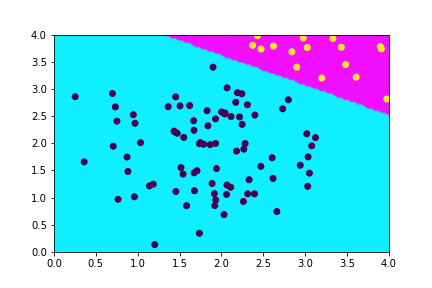
\includegraphics[width=0.8\textwidth]{1a.png}
\end{center}

Polynomial kernel on 2031 dataset. The accuracy after training is 1.0.
\begin{center}
    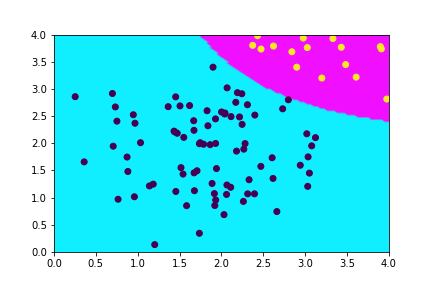
\includegraphics[width=0.8\textwidth]{1b.png}
\end{center}

Gaussian kernel on 2031 dataset with $\sigma=1$. The accuracy after training is 1.0.
\begin{center}
    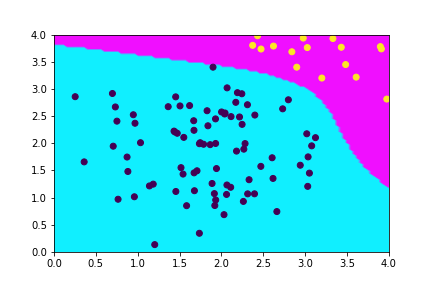
\includegraphics[width=0.8\textwidth]{1c.png}
\end{center}

No-kernel kernel on 2030 dataset gives us accuracy of 0.79, data is linearly separated.
\begin{center}
    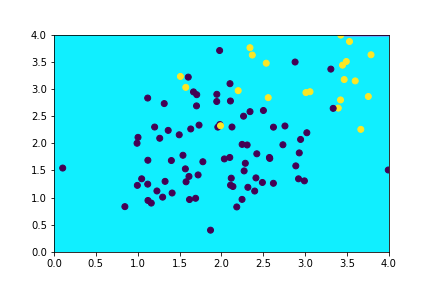
\includegraphics[width=0.8\textwidth]{1di.png}
\end{center}

\newpage Polynomial kernel on 2030 dataset. The accuracy after training is 0.82.
\begin{center}
    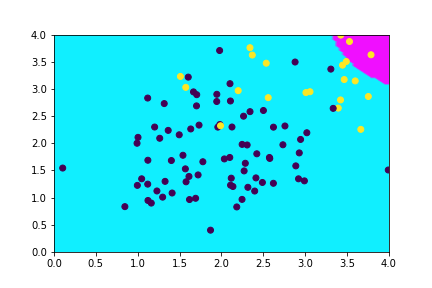
\includegraphics[width=0.8\textwidth]{1dii.png}
\end{center}

Gaussian kernel on 2030 dataset. The accuracy after training is 0.98. Definitely a stranger-looking classifier but it works to cluster a bit.
\begin{center}
    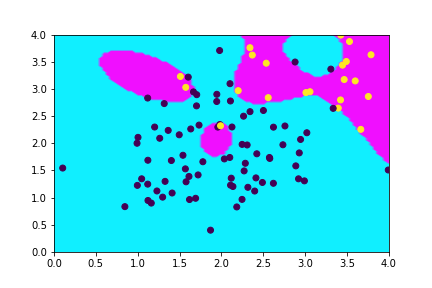
\includegraphics[width=0.8\textwidth]{1diii.png}
\end{center}

\newpage Gaussian kernel on 2030 dataset with $\sigma=3$. The accuracy after training is 1.0. Only this kernel was able to perfectly classify the training dataset on the 2030 data.
\begin{center}
    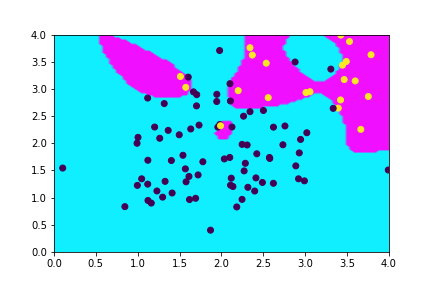
\includegraphics[width=0.8\textwidth]{1div.png}
\end{center}



\question
Conditional probabilities on $C=0$.
\begin{align*}
    P(A|C=0)	&=	P(A=1|C=0)  \\
                &=  0.224 + 0.056   \\
                &=  0.28    \\
    P(B|C=0)    &=	P(B=1|C=0)	\\
                &=	0.024 + 0.056	\\
                &=  0.08    \\
    P(A,B|C=0)  &=  P(A=1, B=1|C=0) \\
                &=  0.056
\end{align*}
Conditional probabilities on $C=1$.
\begin{align*}
    P(A|C=1)	&=	P(A=1|C=1)  \\
                &=  0.27 + 0.03   \\
                &=  0.30    \\
    P(B|C=1)    &=	P(B=1|C=1)	\\
                &=	0.03 + 0.03	\\
                &=  0.06    \\
    P(A,B|C=1)  &=  P(A=1, B=1|C=1) \\
                &=  0.03
\end{align*}
A and B are conditionally independent iff $P(A,B|C) = P(A|C)P(B|C)$. Let's see what it is for each value of C.
\begin{align*}
    P(A,B|C=0)	&?	P(A|C=0)P(B|C=0)	\\
    0.056	&?	0.28 * 0.08	\\
    0.056   &\neq 0.0224    \\
    P(A,B|C=1)	&?	P(A|C=1)P(B|C=1)	\\
    0.03	&?	0.30 * 0.06	\\
    0.056   &\neq 0.018    \\
\end{align*}
A and B are not conditionally independent given C.
\begin{align*}
    P(A)	&=	0.224 + 0.056 + 0.27 + 0.03	\\
            &=  0.58    \\
    P(B)    &=  0.024 + 0.056 + 0.03 + 0.03 \\
            &=  0.14    \\
\end{align*}
A and B are independent if $P(A,B) = P(A)P(B)$.
\begin{align*}
    P(A,B)	&?	P(A)P(B)	\\
    0.056 + 0.03	&?	0.58 * 0.14	\\
    0.086 &\neq 0.0812
\end{align*}
A and B are not independent.


\question
Calculate maximum likelihood estimates.
\begin{align*}
    P(G=1)	&=  6/8	\\
    P(O=1|G=1)  &=    3/6 \\
    P(B=1|G=1)  &=    2/6	\\
    P(C=1|G=1)  &=    3/6 \\
    P(A=1|G=1)  &=    5/6 \\
    P(O=1|G=0)  &=    2/2 \\
    P(B=1|G=0)  &=    2/2	\\
    P(C=1|G=0)  &=    1/2 \\
    P(A=1|G=0)  &=    0/2 \\
\end{align*}

Sample 9 classification. Sample 9 is classified as a good restaurant.
\begin{align*}
    S_1 &=  P(G=1)P(O=0|G=1)P(B=1|G=1)P(C=0|G=1)P(A=1|G=1   \\
        &=  (6/8)(3/6)(2/6)(3/6)(5/6)\\
        &=  0.052   \\
    S_0 &=  P(G=0)P(O=0|G=0)P(B=1|G=0)P(C=0|G=0)P(A=1|G=0   \\
        &=  (2/8)(0/2)(2/2)(1/2)(0/2)\\
        &=  0   \\
\end{align*}

Sample 10 classification. Sample 10 is classified as a good restaurant.
\begin{align*}
    S_1 &=  P(G=1)P(O=1|G=1)P(B=1|G=1)P(C=1|G=1)P(A=1|G=1)   \\
        &=	(6/8)(3/6)  (2/6)  (3/6)  (5/6)	\\
        &=  0.052 \\
    S_0 &=  P(G=0)P(O=1|G=0)P(B=1|G=0)P(C=1|G=0)P(A=1|G=0)   \\
        &=	(2/8)(2/2)  (2/2)  (1/2)  (0/2)	\\
        &=  0 \\
\end{align*}

Calculate maximum likelihood estimates with Laplace smoothing.
\begin{align*}
    P(G=1)	&=  6/8	\\
    P(O=1|G=1)  &=    4/8 \\
    P(B=1|G=1)  &=    3/8	\\
    P(C=1|G=1)  &=    4/8 \\
    P(A=1|G=1)  &=    6/8 \\
    P(O=1|G=0)  &=    3/4 \\
    P(B=1|G=0)  &=    3/4	\\
    P(C=1|G=0)  &=    2/4 \\
    P(A=1|G=0)  &=    1/4 \\
\end{align*}

Sample 9 smoothed classification. Sample 9 is classified as a good restaurant.
\begin{align*}
    S_1 &=  (6/8)(4/8)(3/8)(4/8)(6/8)\\
        &=  0.0527  \\
    S_0 &=  (2/8)(1/4)(3/4)(2/4)(1/4)\\
        &=  0.0058  \\
\end{align*}

Sample 10 smoothed classification. Sample 10 is classified as a good restaurant, but the margin is a bit closer than before.
\begin{align*}
    S_1 &=  (6/8)(4/8)  (3/8)  (4/8)  (6/8)	\\
        &=  0.0527 \\
    S_0 &=  (2/8)(3/4)  (3/4)  (2/4)  (1/4)	\\
        &=  0.0175 \\
\end{align*}


\question
Joint probability of the data.
\begin{align*}
    L	&=	\Pi_i P(x_{ij}, x_{ik}, y_i) 	\\
    L	&=	\Pi_i P(y_i) P(x_{ij}|y_i) P(x_{ik}|y_i) 	\\
    L	&=	\Pi_i (1-\theta_0) \mathbf{1_{y_i=1}} \left(\theta_{j,k|y=1} \theta_{j,s|y=1} \right) + (\theta_0) \mathbf{1_{y_i=0}} \left( \theta_{j,k|y=0} \theta_{j,s|y=0} \right)	\\
    L   &=  \Pi_{y_i = 1} (1-\theta_0 )(\theta_{j,k|y=1} \theta_{j,s|y=1} \Pi_{y_i = 0} (\theta_0) (\theta_{j,k|y=0} \theta_{j,s|y=0})   \\
    N_{y_i = 0} &=  mP(y_i=0)   \\
    N_{y_i = 0} &=  m\theta_0   \\
    L   &=  \boxed{\left[(1-\theta_0) \theta_{j,k|y=1} \theta_{j,s|y=1}\right]^{m(1-\theta_0)} \left[\theta_0 \theta_{j,k|y=0} \theta_{j,s|y=0}\right]^{m\theta_0}}    \\
\end{align*}

\end{document}
